% !TEX TS-program = pdflatex
% !TEX encoding = UTF-8 Unicode

\documentclass[letterpaper, 11pt]{article}

%%%%%%%%%%%%%%%%%%%%%%%%%%%%%%%%%%%%%% %%%%%%%%%%%%%%%%%%%%%%%%%%%%%%%%%%%%%%
%%%%%%%% 패키지 사용 선언 %%%%%%%%%%%%
%% python import와 같은 원리인듯

% layout/spacing related packages
\usepackage[margin=1in]{geometry}
\usepackage{setspace}\onehalfspace
\usepackage{microtype}


% Math related packages
\usepackage{amsmath} \allowdisplaybreaks
\usepackage{amssymb}
\usepackage{amsthm}
%\theoremstyle{definition}    % if you want normal upright font styles for theorems.
\newtheorem{theorem}{Theorem}
\newtheorem{lemma}{Lemma}
\newtheorem{assumption}{Assumption}
\newtheorem{proposition}{Proposition}
\newtheorem{definition}{Definition}


% bibliography and reference related packcages
\usepackage{natbib}
\usepackage{bibentry}
\usepackage{multicol}

\usepackage{booktabs} % for toprule, midrule, bottomrule
\usepackage{graphicx}
\usepackage{appendix}
\usepackage[counterclockwise]{rotating} % for sidewaystable
\usepackage{subcaption} % for subfigure
\usepackage[normalem]{ulem} % for uline
\usepackage{showexpl}
\usepackage{threeparttable} % for tables with footnotes

\usepackage[hyphens]{url}
\usepackage[bookmarks=false,hidelinks]{hyperref}

\usepackage{tikz}
\usetikzlibrary{automata,calc,trees,positioning,arrows,chains,shapes.geometric,%
decorations.pathreplacing,decorations.pathmorphing,shapes,%
matrix,shapes.symbols,plotmarks,decorations.markings,shadows}

\usepackage{pgf}
\pgfdeclarelayer{background}
\pgfdeclarelayer{foreground}
\pgfsetlayers{background,main,foreground}


\usepackage{authblk}
\renewcommand\Authfont{\sf\Large}
\renewcommand\Affilfont{\rm\small}
 %%%%%%%%%%%%%%%%%%%%%%%%%%%%%%%%%%%%%% %%%%%%%%%%%%%%%%%%%%%%%%%%%%%%%%%%%%%%



%%%%%%%%%%%%%%%%%%%%%%%%%%%%%%%%%%%%%% %%%%%%%%%%%%%%%%%%%%%%%%%%%%%%%%%%%%%%
%%%%%%%%%%%%%% MACRO %%%%%%%%%%%%%%%%%%%%%%%%%%%%%%%%%%%%%%
%% 자주 사용하는 단어들을 매크로로 지정한다.
%% 일일이 오퍼레이터를 사용안하고 메크로를 통해 더 자유롭게 사용.
\newcommand{\email}[1]{{\href{mailto:#1}{\nolinkurl{#1}}}}

\usepackage{bm}
\renewcommand{\vec}[1]{\boldsymbol{\mathbf{#1}}}
\newcommand{\mat}[1]{\vec{#1}}
\newcommand{\set}[1]{\mathcal{#1}}

% https://tex.stackexchange.com/questions/265689/ignore-greek-letters-using-mathcal
\DeclareMathSymbol{\Gamma}{\mathord}{operators}{"00}
\DeclareMathSymbol{\Delta}{\mathord}{operators}{"01}
\DeclareMathSymbol{\Theta}{\mathord}{operators}{"02}
\DeclareMathSymbol{\Lambda}{\mathord}{operators}{"03}
\DeclareMathSymbol{\Xi}{\mathord}{operators}{"04}
\DeclareMathSymbol{\Pi}{\mathord}{operators}{"05}
\DeclareMathSymbol{\Sigma}{\mathord}{operators}{"06}
\DeclareMathSymbol{\Upsilon}{\mathord}{operators}{"07}
\DeclareMathSymbol{\Phi}{\mathord}{operators}{"08}
\DeclareMathSymbol{\Psi}{\mathord}{operators}{"09}
\DeclareMathSymbol{\Omega}{\mathord}{operators}{"0A}

\newcommand{\LB}{\mathsf{LB}}
\newcommand{\UB}{\mathsf{UB}}		

\usepackage{xcolor}
\newcommand{\note}[1]{{\Large\bf#1}}
\newcommand{\bluenote}[1]{{\Large\color{blue}#1}}
\newcommand{\rednote}[1]{{\Large\color{red}#1}}

\usepackage{etoolbox}
% To use, for example, \Ac for \mathcal{A}.  Requires "etoolbox" package
\makeatletter
\def\do#1{\@namedef{#1c}{\ensuremath{\mathcal{#1}}}}
\docsvlist{A,B,C,D,E,F,G,H,I,J,K,L,M,N,O,P,Q,R,S,T,U,V,W,X,Y,Z}
\makeatother

\def\Eb{\mathbb{E}}
\def\Rb{\mathbb{R}}
%\def\response{[$\Longrightarrow$]}

\newenvironment{response}
{ [$\Longrightarrow$]\sf }
{ \hfill \rule{1ex}{1ex} }

\newcommand{\dx}{\mathop{}\!\mathrm{d}x}
\newcommand{\dy}{\mathop{}\!\mathrm{d}y}
\newcommand{\dz}{\mathop{}\!\mathrm{d}z}
\newcommand{\dt}{\mathop{}\!\mathrm{d}t}

\renewcommand{\bar}[1]{\mkern 1.5mu\overline{\mkern-1.5mu#1\mkern-1.5mu}\mkern 1.5mu}



%%%%%%%%%%%%%%%%%%%%%%%%%%%%%%%%%%%%%% %%%%%%%%%%%%%%%%%%%%%%%%%%%%%%%%%%%%%%
% To show LaTeX code examples

\usepackage{fancyvrb,listings}
\lstset{
   breaklines=true,
   basicstyle=\linespread{0.8}\ttfamily\scriptsize,
   aboveskip=0pt,
   belowskip=0pt
}
\newenvironment{example}
 {\VerbatimOut{\jobname.tmp}}
 {\endVerbatimOut
 \begin{center}
 \fbox{
	 \begin{minipage}[c]{0.48\textwidth}
	  \lstinputlisting{\jobname.tmp}
	 \end{minipage}
   }
 \fbox{
 	\begin{minipage}[c]{0.38\textwidth}
 	 \scriptsize
	 \input{\jobname.tmp}
  	\end{minipage}
  }
  \end{center}
 }

%%%%%%%%%%%%%%%%%%%%%%%%%%%%%%%%%%%%%%%%%%%%%%%%%%%%%%%%





\title{[COMP6245 Foundation of Machine Learning] \\ LabOne: Multi-variate Gaussian}
\author{31240232 / Sunwung Lee}
\affil{MSc Artificial Intelligence, University of Southampton}

\date{14 October 2019}

%\usepackage{showlabels}
%\usepackage[final]{showlabels}


\begin{document}
\maketitle
\section{Linear Algebra}

The last line of the advanced topic, singular value decomposition(SVD) example code $\mat{U}\mat{U^T}$, is identified an identity matrix($\mat{I}$). $\mat{U}$ is the eigenvector matrix of $\mat{B}$, and the result of $\mat{U}\mat{U^T}$ must be an orthogonal matrix because it is an identity matrix. 
Next, SVD can be expressed by the following formula.

\begin{center}
    
$\mat{A}=\mat{U}\mat{\Sigma}\mat{V^T}$

$\mat{A} = m\times n \; \texttt{Rectangular matrix}, \quad  \mat{U} = m\times m \; \texttt{orthogonal matrix}$ \\
$\mat{\Sigma} = m\times n \; \texttt{diagonal matrix}, \quad \mat{V^T} = n\times n \; \texttt{orthogonal matrix}$

\end{center}
The great advantage of SVD is that it can be used widely for all rectangular matrices of $m\times n$ consisting of real or complex spatial elements. In addition, SVD allows arbitrary $\mat{A}$ to be divided into layers based on the amount of information.
Finally, the size of $\mat{B}$ is predictable. 1) The determinant is not 0. 2) There is an inverse matrix. 3) There are 3 eigenvalues. 4) rank = 3.\\
Therefore, $\mat{B}$ is a $3\times 3$ square matrix.

\section{Random Numbers and Univariate Distributions}

First of all, briefly, the definitions of the rand and randn functions.
\begin{center}
1) rand: Create an array of the given shape it with random samples from a uniform distribution.\\
2) randn: Return a sample (or samples) from the “standard normal” distribution.
\end{center}
\begin{figure}[h] %%% t: top, b: bottom, h: here
\centering
\subfigure[]{

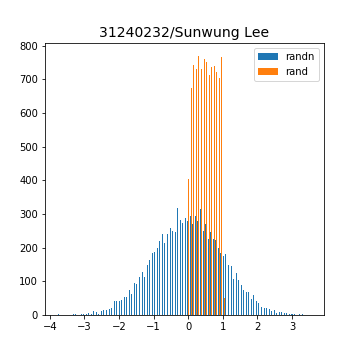
\includegraphics[width=0.3\linewidth]{2_rand_randn.png}
\hspace{0.5cm}
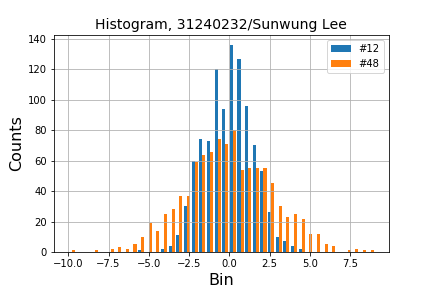
\includegraphics[width=0.45\linewidth]{2_rand_randn_2.png}
\caption{L: difference between rand, randn / R: change of histogram according to random numbers}

}
\end{figure}
This can be confirmed by histogram. However, the appearance of this histogram depends on the number of bins and the number of samples.
An important parameter of the hist function, bins, is defined as "int or sequence or str, optional. if an integer is given, bins + 1 bin edges are calculated and returned consistent with numpy.histogram", which provides an accurate view of the data in histogram.\\
In addition, as the number of samples increases, the features of rand and randn functions become more apparent.
For example, in the case of randn, the larger the number of samples, the more clearly the normal distribution with a mean of 0 and a standard deviation of 1 can be identified.

\noindent Through Figure 1 it can certainly compare the features of the rand and randn functions. Histogram shows the following difference. A histogram was drawn using the difference of the sum of the random variables through the rand function. Naturally, the larger the total number of repetitions, N, the clearer the normal distribution curve. If uniform random number(URN) is $12$, the mean is close to $0$ and the standard deviation has $\sqrt{2}$. However, if the URN is getting larger, the standard deviation increases. Conversely, the smaller the standard deviation approaches zero.

\section{Uncertainty in Estimation}

The smaller the number of arbitrary variables xx, defined as xx in code, the greater the value of the variance. This is because it is not a sufficient number of variables that cannot draw a normal distribution tendency.
\begin{figure}[h] %%% t: top, b: bottom, h: here

\begin{center}

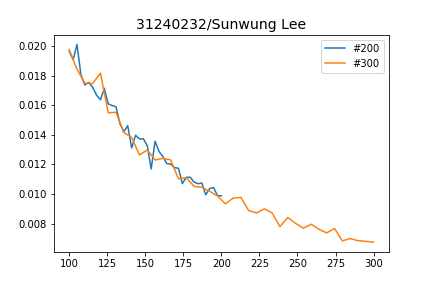
\includegraphics[width=0.5\linewidth]{3_Uncertainty_in_Estimation.png}
\caption{Uncertainty in Estimation}
\end{center}
\end{figure}
In addition, the variance of the variances of arbitrary variable values can be analyzed. In other words, a small variance value of the variances means that when the same number of data is repeated n times, the resulting data converges further to the mean value. In the same way, this means that xx better represents a normal distribution. \\
This can be expected to hold the greater amount of data and to better catch the characteristics of that data.

 

\section{Bivariate Gaussian Distribution}

Why should Bivariate Gaussian Distribution use? Suppose there are two variables in the dataset $(x_1, x_2)$, where $x_1$ is normally distributed and $x_2$ is also normally distributed. In this case, exception data may be wrongly judged. To avoid this, multivariate Gaussian distributions are used. For example, in the Bivraiate Gaussian Distribution, a researcher can check the distribution of variables for students' height $(x_1)$, weight $(x_1)$, and  $(x_1, x_2)$ following a normal distribution. \\
Let's look at the function part of the example python code.\\
Gauss2D(x, m, $\mat{C}$): The return value follows the mean $m$, variance $\mat{C}$ in Gaussian equation.
Moreover, contours represent groups of the same level. Use the meshgrid function in python to draw this.
\begin{figure}[h] %%% t: top, b: bottom, h: here
\centering
\subfigure[]{

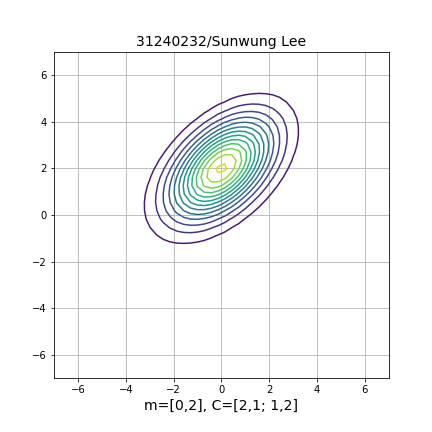
\includegraphics[width=0.3\linewidth]{4_Bivariate_Gaussian_Distribution-1.png}
\hspace{0.5cm}
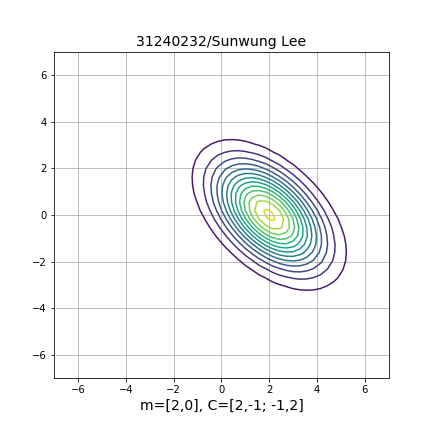
\includegraphics[width=0.3\linewidth]{4_Bivariate_Gaussian_Distribution-2.png}
\hspace{0.5cm}
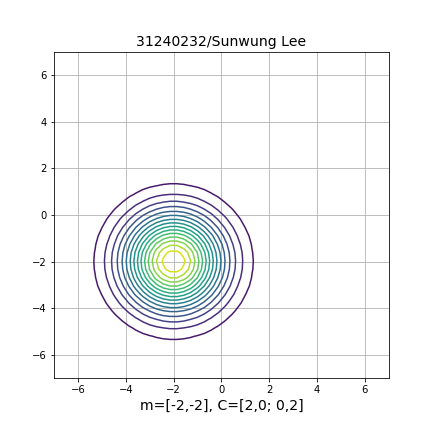
\includegraphics[width=0.3\linewidth]{4_Bivariate_Gaussian_Distribution-3.png}
\caption{Examples of bivariate Gaussian distribution}
}

\end{figure}

\noindent The figure above shows the results of experiments using three different examples of means($m$) and covariance matrices($\mat{C}$) using the contour function.
The centre of the ellipse / circle is determined by $m$, and the direction of the ellipse is determined by the value of the $\mat{C}$.

\section{Sampling from a Multivariate Gaussian Distribution}
The covariance matrix($\mat{C}$) can be expressed as the product of the lower triangular matrix($\mat{A}$), by Cholesky decomposition.
The Python example code generates a random number($\mat{X}$) that follows a normal distribution, and $\mat{Y}$ is expressed as the product of $\mat{X}$ and $\mat{A}$.
The reason for decomposing a matrix by Cholesky decomposition is to make the calculation more convenient. This simplifies the system matrix and makes it easier to analyze.

\begin{figure}[h] %%% t: top, b: bottom, h: here

\begin{center}

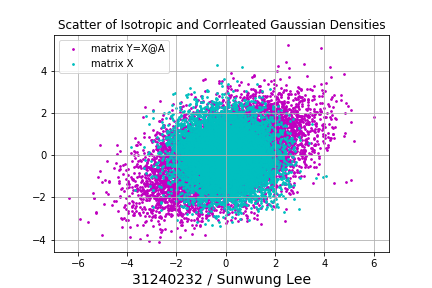
\includegraphics[width=0.5\linewidth]{5_Sampling_from_a_Multivariate_Gaussian_Distribution.png}
\caption{Scatter plot of $\mat{X}$ and $\mat{Y}$($=\mat{X}\mat{A}$)}
\end{center}
\end{figure}
The code results show that multiplying $\mat{A}$ and $\mat{X}$ gives the effect of $\mat{C}$ on $\mat{X}$ and the shape of data changes ellipse.

\section{Distribution of Projections}

In the Python example code, thRange is set to 50 divided by 0 to $2\pi$. In addition, theta is each divided by 50, which constitutes a $\mat{u}$. The pVars array stores the variance of the values of the projection of the $\mat{Y}$ onto the vector $\mat{u}$.

\begin{figure}[h] %%% t: top, b: bottom, h: here
\centering
\subfigure[]{

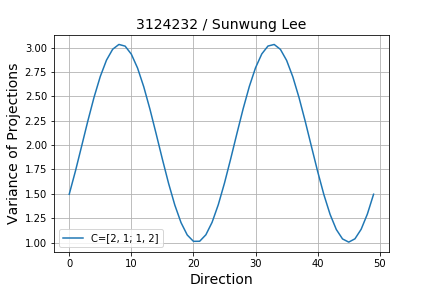
\includegraphics[width=0.4\linewidth]{6_Distribution_of_Projection-1.png}
\hspace{0.5cm}
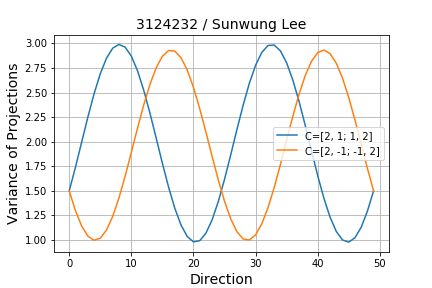
\includegraphics[width=0.4\linewidth]{6_Distribution_of_Projection-2.png}
\caption{Examples of distribution of projection}
}

\end{figure}
As you can see on the left figure, the value of pVars is represented in the form of a sine function.
The calculation shows that the covariance matrix has eigenvalues of 3 and 1, so eigenvectors can find two vectors, $x_2 = x_1$ and $x_2 = -x_1$.\\
In addition, $\mat{C}=$ \begin{bmatrix}
2 & -1\\ 
-1 & 2
\end{bmatrix}, the phase of the sine waveform is changed, and when the two graphs are drawn at the same time, it appears on the right figure.

\end{document}







%
